% chapter 1 section 1

\section{运动与力}

\subsection{速度与加速度}

\subsubsection{直线运动}

\begin{figure}[ht!]
    \centering
    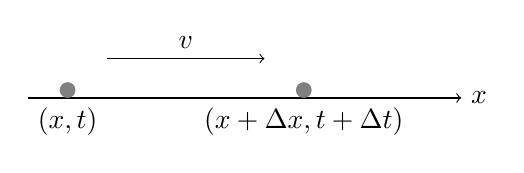
\begin{tikzpicture}
        \draw[->] (-0.5, 0) -- (5, 0) node[right] {$x$};
        \fill[fill=gray] (0, 0.1) circle (0.1);
        \node[below] at (0, 0) {$(x, t)$};
        \fill[fill=gray] (3, 0.1) circle (0.1);
        \node[below] at (3, 0) {$(x+\Delta x, t+\Delta t)$};
        \draw[->] (0.5, 0.5) -- node[above] {$v$} (2.5, 0.5);
    \end{tikzpicture}
    \caption{速度与时间}
\end{figure}

\paragraph{速度}对于在x轴上运动的物体,其在这段时间内的平均速度可如下给出:
\begin{equation*}
    \bar{v} = \frac{\Delta x}{\Delta t}
\end{equation*}
其中$\Delta x$的部分叫做変位,其方向为初始位置指向终止位置。当这个时间间隔无限趋于0时,将这个极限值称为(瞬时)速度,即:
\begin{equation*}
    v = \lim_{\Delta t\to0}\frac{\Delta x}{\Delta t}=\frac{dx}{dt}
\end{equation*}
速度的方向由变位的方向决定,单位常用$\left(m/s\right)$。其大小可以用:速度の大きさ、速さ等词汇描述。

\paragraph{加速度}与速度类似,当我们着眼于某个时间间隔内速度的变化时,便可以得到平均加速度的定义。若再将其时间间隔无限缩小至0就有了(瞬时)加速度:
\begin{equation*}
    a = \lim_{\Delta t\to0}\frac{\Delta v}{\Delta t}=\frac{dv}{dt}
\end{equation*}
同样的,由于速度是矢量所以加速度也是具有方向的,其方向取决于速度变化的方向,单位常用$\left(m/s^2\right)$。

\paragraph{图像表示}在$v-t$图像中,根据速度定义可知:
\begin{equation*}
    \textrm{变位的(微小)变化}=\textrm{速度}\times\textrm{时间的(微小)变化}
\end{equation*}
所以,数形结合可得$v-t$图像与时间轴围成的面积即为该时间间隔内物体的距离。但有些时候围成的图形会跨过时间轴,此时根据速度值的正负(方向)可分析得到:横轴以上的面积表示正方向上的距离,横轴以下的部分表示负方向上的距离。
\begin{figure}[ht!]
    \centering
    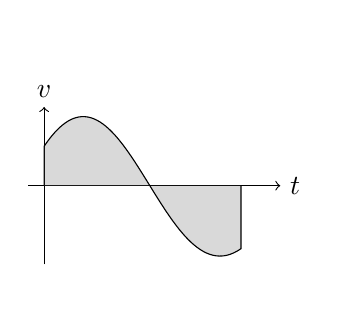
\begin{tikzpicture}
        \draw[->] (-0.2, 0) -- (3, 0) node[right] {$t$};
        \draw[->] (0, -1) -- (0, 1) node[above] {$v$};
        \filldraw[color=black, fill=gray, fill opacity=0.3] (0, 0) -- 
            (0, 0.5) .. controls (1, 2) and (1.5, -1.5) .. (2.5, -0.8) -- (2.5, 0);
    \end{tikzpicture}
    \caption{$v-t$图像}
\end{figure}
此外,根据加速度的定义,我们可以根据$v-t$图像的斜率来确定其值。
\begin{itemize}
    \item 图形面积$\implies$移动距离
    \item 切线斜率$\implies$加速度
\end{itemize}

\paragraph{等加速度直线运动}加速度一定的直线运动,属于最基本的运动类型。
\begin{figure}[ht!]
    \centering
    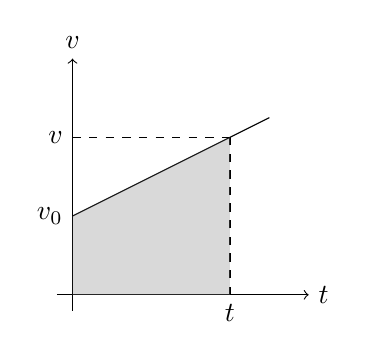
\begin{tikzpicture}
        \draw[->] (-0.2, 0) -- (3, 0) node[right] {$t$};
        \draw[->] (0, -0.2) -- (0, 3) node[above] {$v$};
        \draw[domain=0:2.5] plot (\x, {0.5*\x + 1});
        \coordinate[label=left:$v$] (v) at (0, 2);
        \coordinate[label=left:$v_0$] (v0) at (0, 1);
        \coordinate[label=below:$t$] (t) at (2, 0);
        \draw[dashed] (v) -- (2, 2);
        \draw[dashed] (t) -- (2, 2);
        \fill[fill=gray, opacity=0.3] (0, 0) -- (v0) -- (2, 2) -- (t) --cycle;
    \end{tikzpicture}
    \caption{等加速度直线运动图像}
\end{figure}

\begin{itembox}[l]{运动学基本公式}
    \begin{gather*}
        v=v_0+at\\
        x=v_0t+\frac{1}{2}at^2\\
        v^2-{v_0}^2=2ax
    \end{gather*}
\end{itembox}

\subsubsection{平面运动分析}

根据速度/加速度的矢量性,运动可以轻松地被扩展到平面上。而且倘若借助向量、坐标等数学手段,我们就可以驾驭更加复杂的运动形式。
\begin{figure}[ht!]
    \centering
    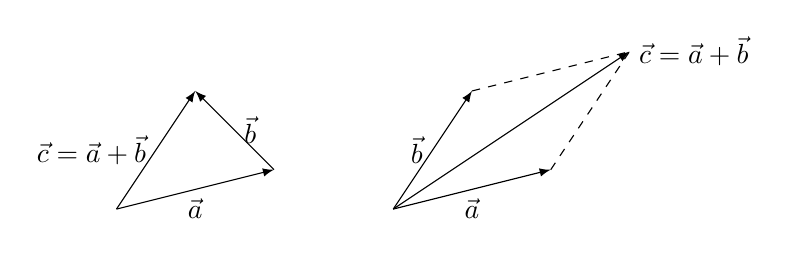
\begin{tikzpicture}
        \begin{scope}
            \draw[-latex] (0, 0) -- node[below] {$\vec{a}$} (2, 0.5);
            \draw[-latex] (2, 0.5) -- node[right] {$\vec{b}$} (1, 1.5);
            \draw[-latex] (0, 0) -- node[left] {$\vec{c}=\vec{a}+\vec{b}$} (1, 1.5);
        \end{scope}
        \begin{scope}[xshift=100pt]
            \draw[-latex] (0, 0) -- node[below] {$\vec{a}$} (2, 0.5);
            \draw[-latex] (0, 0) -- node[left] {$\vec{b}$} (1, 1.5);
            \draw[-latex] (0, 0) -- (3, 2) node[right] {$\vec{c}=\vec{a}+\vec{b}$};
            \draw[dashed] (2, 0.5) -- (3, 2);
            \draw[dashed] (1, 1.5) -- (3, 2);
        \end{scope}
    \end{tikzpicture}
    \caption{向量合成与分解}
\end{figure}
如果将上述的合成与分解放到平面直角坐标系内操作,就是最常见也最常用的形式。
\begin{figure}[ht!]
    \centering
    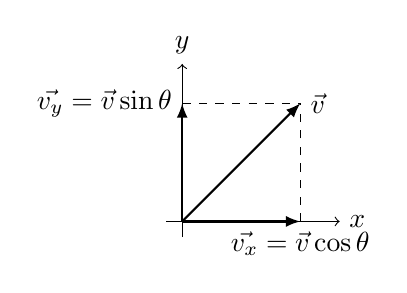
\begin{tikzpicture}
        \draw[->] (-0.2, 0) -- (2, 0) node[right] {$x$};
        \draw[->] (0, -0.2) -- (0, 2) node[above] {$y$};
        \draw[thick, -latex] (0, 0) -- (1.5, 1.5) node[right] {$\vec{v}$};
        \draw[thick, -latex] (0, 0) -- (1.5, 0) node[below] {$\vec{v_x}=\vec{v}\cos\theta$};
        \draw[thick, -latex] (0, 0) -- (0, 1.5) node[left] {$\vec{v_y}=\vec{v}\sin\theta$};
        \draw[dashed] (1.5, 0) -- (1.5, 1.5);
        \draw[dashed] (0, 1.5) -- (1.5, 1.5);
        \drawangle{(1, 0)}{(0, 0)}{(1, 1)};
    \end{tikzpicture}
    \caption{速度的正交分解}
\end{figure}
\begin{itembox}[l]{运动分析}
    \begin{itemize}
        \item 合成分解:$\vec{v}\rightleftharpoons\vec{v_1}+\vec{v_2}$
        \item 相对速度:$\textrm{相对}=\textrm{对象}-\textrm{参考/基准}$
    \end{itemize}
\end{itembox}

\subsection{运动与力}

\subsubsection{力}

力的三要素(力的大小、作用线、作用点)、单位(N)等内容比较基础,在此略过。

\paragraph{力的平衡}由于力也是矢量,所以我们也可以对其进行合成/分解的操作。一般称合成得来的力为合力,称分解得来的力为分力。在考虑受力平衡时便借助此思想,将某物体视为质点\footnote{忽略极小或质量分布均匀的物体的大小,将其视作一个点。},其合力为0的状态定义为平衡状态。个人常用$\sum\vec F=0$的方式来简记。

\paragraph{重力}吸引地表所有物体,竖直向下的力。其成因是万有引力。数学形式为:$G=m\cdot g$。

\paragraph{张力/拉力}一般指绳子上的张力或拉力。对于轻质绳子,\underline{同一条绳子}上的拉力处处相等

\paragraph{弹力}日文为弾性力,指的是弹簧为了恢复到\underline{自然长/原长}而产生的力。弹力遵循胡克定律,日文为フックの法則。使用时应注意形变量具有方向。
\begin{itembox}[l]{胡克定律}
    \begin{equation*}
        \vec{F}=-k\vec{\Delta x}\quad(k:\textrm{バネ定数},\Delta x:\textrm{基于原长的形变量})
    \end{equation*}
\end{itembox}
\begin{figure}[ht!]
    \centering
    \begin{tikzpicture}
        \fill[fill=gray, opacity=0.3] (0, 0.2) rectangle (6, 0);
        \draw (0, 0) -- (6, 0); 
        \draw[spring] (1, 0) -- ++ (0, -1.6);
        \fill[fill=black] (1, -1.6) circle (3pt);
        \draw[spring] (3, 0) -- ++ (0, -1.6);
        \draw[spring] (3, -1.6) -- ++ (0, -1.6);
        \fill[fill=black] (3, -3.2) circle (3pt);
        \draw[spring] (4.8, 0) -- ++ (0, -1.3);
        \draw[spring] (5.3, 0) -- ++ (0, -1.3);
        \draw (4.8, -1.3) -- (5.3, -1.3);
        \draw (5.05, -1.3) -- (5.05, -1.5);
        \fill[fill=black] (5.05, -1.5) circle (3pt);
    \end{tikzpicture}
    \caption{弹簧串并联}
\end{figure}
\begin{itembox}[l]{弹簧串并联}
    \begin{itemize}
        \item 串联(受力一致)
        \begin{equation*}
            \begin{cases}
                F=k_1x_1=k_2x_2\\
                F=K(x_1+x_2)
            \end{cases}\implies\frac1K=\frac1{k_1}+\frac1{k_2}
        \end{equation*}
        \item 并联(形变一致)
        \begin{equation*}
            \begin{cases}
                F=F_1+F_2=k_1x+k_2x\\F=Kx
            \end{cases}\implies K=k_1+k_2
        \end{equation*}
    \end{itemize}
\end{itembox}

\paragraph{摩擦力}摩擦力来自于物体和接触面之间的支持力,日文为垂直抗力。应明确接触为要因,有接触则会产生支持力,进而才涉及摩擦力问题。其数学形式为:$f=N\cdot\mu$,其中$\mu$为摩擦系数。
\begin{figure}[ht!]
    \centering
    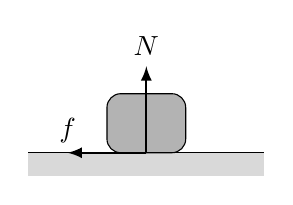
\begin{tikzpicture}
        \draw (0, 0) -- (3, 0);
        \fill[fill=gray, opacity=0.3] (0, 0) rectangle (3, -0.3);
        \filldraw[color=black, fill=gray, fill opacity=0.6, rounded corners=5pt] (1, 0) rectangle (2, 0.75);
        \draw[-latex, thick] (1.5, 0) -- (1.5, 1.1) node[above] {$N$};
        \draw[-latex, thick] (1.5, 0) -- (0.5, 0) node[above] {$f$};
    \end{tikzpicture}
    \caption{摩擦力}
\end{figure}
如果给一个物体施加一个线性变大的力,作用在其身上的摩擦力变化如图。
\begin{figure}[ht!]
    \centering
    \begin{tikzpicture}
        \draw[->] (-0.2, 0) -- (3, 0) node[right] {$t$};
        \draw[->] (0, -0.2) -- (0, 3) node[above] {$f$};
        \draw[thick] (0, 0) -- (1, 2) node[above, fill=white]{$f_0=N\cdot\mu\quad(\mu:\textrm{静止摩擦系数})$};
        \draw[thick] (1, 2) -- (1, 1.5);
        \draw[thick] (1, 1.5) -- (3, 1.5) node[right] {$f=N\cdot\mu^\prime\quad(\mu^\prime:\textrm{滑动摩擦系数})$};
    \end{tikzpicture}
    \caption{摩擦力变化}
\end{figure}
由此可知,静止摩擦力是物体在发生运动之前用来平衡外力的力,其最大值是最大静摩擦力。

\subsubsection{运动法则}

\begin{itembox}[l]{牛顿运动定律}
    \begin{itemize}
        \item 惯性法则:物体\underline{不受力}或\underline{合外力为0}时,运动状态不发生改变(惯性)。
        \item 运动法则:物体受力后会产生与力\underline{同方向}的加速度。加速度大小与力的大小成正比,与物体质量成反比。
        \begin{equation*}
            \vec{a}=k\cdot\frac{\vec{F}}{m}\to
            \vec{F}=m\vec{a}
        \end{equation*}
        \item 作用力与反作用力法则:物体A向物体B施力后,会受到来自物体B的\underline{大小相等}、\underline{方向相反}(等大反向)的力。
    \end{itemize}
\end{itembox}
其中惯性法则揭示的本质问题是:力是改变物体运动状态的原因。同时应注意,作用力与反作用力的分析对象为两个物体,而受力平衡则只针对单个物体论。

\subsubsection{重力相关的运动}

\paragraph{落体运动}根据物体的初速度有以下三种情况。
\begin{itemize}
    \item 自由落体:初速度为0,只受重力。
    \item 上抛运动:初速度向上为$v_0$,只受重力。
    \item 下抛运动:初速度向下为$v_0$,只受重力。
\end{itemize}
将上述条件代入运动学基本公式就可得该特殊情形下的运动方程。
\begin{itembox}[l]{自由落体}
    \begin{equation*}
        \begin{cases}
            v=gt\\
            h=\frac{1}{2}gt^2\\
            v^2=2gh
        \end{cases}
    \end{equation*}
\end{itembox}

\paragraph{抛体运动}将落体运动扩展到平面内得到的便是抛体运动。
\begin{figure}[ht!]
    \centering
    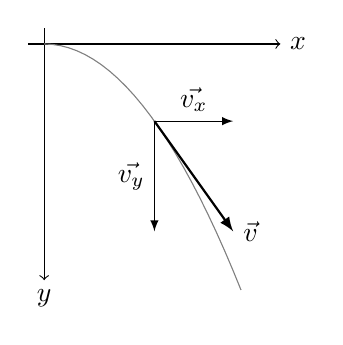
\begin{tikzpicture}
        \draw[->] (-0.2, 0) -- (3, 0) node[right] {$x$};
        \draw[->] (0, 0.2) -- (0, -3) node[below] {$y$};
        \draw[color=gray, domain=0:2.5] plot (\x, {-0.5*\x^2});
        \draw[thick, -latex] (1.4, -0.98) -- (2.4, -2.38) node[right] {$\vec{v}$};
        \draw[-latex] (1.4, -0.98) -- node[above] {$\vec{v_x}$} (2.4, -0.98);
        \draw[-latex] (1.4, -0.98) -- node[left] {$\vec{v_y}$} (1.4, -2.38);
    \end{tikzpicture}
    \caption{平抛运动}
\end{figure}
\subparagraph{平抛运动}
\begin{itemize}
    \item 条件:水平初速度为$v_0$,只受重力。
    \item 分析:
    \begin{equation*}
        \begin{cases}
            \textrm{水平}:a_x=0\implies\textrm{匀速直线运动}\\
            \textrm{竖直}:a_y=g\implies\textrm{自由落体}
        \end{cases}
    \end{equation*}
\end{itemize}

\begin{figure}[ht!]
    \centering
    \begin{tikzpicture}
        \draw[->] (-0.2, 0) -- (5, 0) node[right] {$x$};
        \draw[->] (0, -0.2) -- (0, 2.5) node[above] {$y$};
        \draw[color=gray, domain=0:4] plot (\x, {-0.5*(\x-2)^2+2});
        \draw[thick, -latex] (0, 0) -- (0.5, 1) node[above] {$v_0$};
        \drawangle{(1, 0)}{(0, 0)}{(1, 2)};
        \draw[dashed] (2, 2) -- (2, 0) node[below] {$x_{mid}$};
        \draw[dashed] (2, 2) -- (0, 2) node[left] {$y_{max}$};
        \node[below] at (4, 0) {$x_{max}$};
    \end{tikzpicture}
    \caption{斜抛运动}
\end{figure}
\subparagraph{斜抛运动}
\begin{itemize}
    \item 条件:初速度为$v_0$,倾角$\theta$,只受重力。
    \item 分析:
    \begin{equation*}
        \begin{cases}
            \textrm{水平:初速度}v_0\cos\theta,\textrm{不受力}\implies\textrm{匀速直线运动}\\
            \textrm{竖直:初速度}v_0\sin\theta,\textrm{受重力}\implies\textrm{上抛运动}
        \end{cases}
    \end{equation*}
    \item 结论1:纵向最大高度
    \begin{gather*}
        \begin{cases}
            v=v_0\sin\theta-gt\\
            y=v_0\sin\theta t-\frac{1}{2}gt^2
        \end{cases}\\
        v=0,\textrm{即}t=\frac{v_0\sin{\theta}}{g}\textrm{时}
        y=\frac{{v_0}^2\sin^2{\theta}}{2g}\textrm{最高}
    \end{gather*}
    \item 结论2:滞空时间
    \begin{equation*}
        y=0\implies t=0,\frac{2v_0\sin{\theta}}{g}\textrm{(对称)}
    \end{equation*}
    \item 结论3:最远距离
    \begin{gather*}
        x=v_0\cos{\theta}\frac{2v_0\sin\theta}{g}=\frac{{v_0}^2\sin{2\theta}}{g}\\
        \therefore\theta=45^\circ\textrm{时},x=\frac{{v_0}^2}{g}\textrm{最大}
        \end{gather*}
\end{itemize}

\subsection{刚体与力}

\subsubsection{刚体}

与质点类似,刚体也是为分析方便而引入的一种理想模型。对于一般物体来说当受力时不可避免地会产生些许形变,然而处理大多数问题的过程中,这些形变无关紧要。那么,不考虑受力形变的刚体便应运而生。

\subsubsection{力矩}

日文为力のモーメント,是一种描述物体绕轴旋转情况的物理量。标准定义为力臂(腕の長さ)和力的向量积\footnote{力矩:$\vec{M}=\vec{r}\times\vec{F}$}。因此力矩是一个矢量,由旋转方向和旋转的强度构成,但解题时常常将这两个信息分开考虑。
\begin{figure}[ht!]
    \centering
    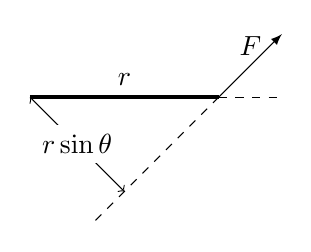
\begin{tikzpicture}[scale=0.8]
        \draw[ultra thick] (0, 0) -- node[above] {$r$} (3, 0);
        \draw[-latex] (3, 0) -- node[above] {$F$} (4, 1);
        \draw[dashed] (3, 0) -- (4, 0);
        \drawangle{(4, 0)}{(3, 0)}{(4, 1)};
        \draw[dashed] (3, 0) -- (1, -2);
        \draw[<->] (0, 0) -- node[fill=white] {$r\sin\theta$} (1.5, -1.5);
    \end{tikzpicture}
    \caption{力矩}
\end{figure}
\begin{itembox}[l]{力矩}
    \begin{equation*}
        M=F\cdot r\cdot\sin\theta
    \end{equation*}
\end{itembox}

\subsubsection{非共点力刚体平衡}

在考虑刚体平衡时,除了需要满足牛顿第一定律的条件以外,还需要保证物体自身不能旋转,即力矩平衡。
\begin{itembox}[l]{刚体平衡条件}
    \begin{itemize}
        \item 受力平衡:$\sum\vec{F}=0$
        \item 力矩平衡:$\sum\vec{M}=0$
    \end{itemize}
\end{itembox}
因此,在刚体上做力的合成时需要确保其总力矩不发生改变。
